\chapter{Experiment and Results}

\section{Data}
There are 450 videos in two formats, avi and flv, 89 of them are flv videos, 361 of them are avi videos. The time of videos are from seconds to dozens of seconds. Videos were recorded using web-cam of different PCs. Video background are vary as the video are recorded in a place chosen by subject. People are free to do anything while recording the video, I even observe a male disappear from the camera for half of the video sequence while recording. As a result, there are no faces in most of the video frames. The Intraface tracker \cite{xiong2013supervised} is used to track those videos. It is able to track 439 videos. 1 video is tracked, but the tracking result does not match the label. 10 videos are tracked, but unable to identify the face in the video. The face in those untracked video can be clear identify by visual. One possible may be the resolution of the image. Maximum untracked video frame is $240*960$ pixels. Minimum tracked video frame size is $240*960$, the same as the maximum size of untracked video frame. It is reasonable to say tracker \cite{xiong2013supervised} may not be good at tracking low resolution videos. The observation mentioned in comparing tracker \cite{xiong2013supervised} and tracker \cite{asthana2013robust} also support this hypothesis. The maximum frame tracked is $600*2400$. For each video there is a label file indicate the label of each frame, The frame number of each video is quite different, from around 200 to more than 900. The frame rate is 30 fps. Table\ref{tab:TR} shows the tracking result of tracker \cite{xiong2013supervised}.
\begin{table}[ht]
\begin{tabular}{|l|*{6}{c|}}
\hline
\diagbox{Title}{Label} & Normal Face & Eating & Talking & Looking Away & Occluded & Other Problem \\ \hline
Total   & 35361       & 10409  & 5623    & 7730         & 21394    & 8422          \\ \hline
Tracked & 33776       & 9460   & 5196    & 5405         & 19014    & 3884          \\ \hline   
Rate		& 0.9552      & 0.9088 & 0.9241  & 0.6992       & 0.8888   & 0.4612        \\ \hline
\end{tabular}
\caption{Frame tracking result by tracker \cite{xiong2013supervised}}
\label{tab:TR}
\end{table}
\newline
There are six labels for each frame, normal face, eating, talking, looking away, occluded, other problem. A frame labelled as eating belong to a image sequence of eating. Label normal face, eating, talking and looking away are disjoint, but one frame can be labelled as one of them and occluded or other problem. It is very hard to track a face that face to camera from a certain angle, so the tracking rate is very small for a face looking away. I only use frame with label normal face, eating, talking in the experiment. Not all three labels are included in all videos, most of videos miss one or two or even all three labels.
\subsection{Feature}
Each face is aligned with 49 facial feature points as shown in figure \ref{fig:IPI}. As the tracker doesn't provide face bound point, so I am unable to include jaw and cheek in the ROI. I just kept the mouth as Region of Interest. I extract Local Binary Pattern feature from ROI. The size appearance feature vector are different if I divide image of ROI into different number of blocks. I tried dividing ROI into 1 block and $1*3$ blocks, size of appearance feature vector is 95 and 177. As there are 49 shape feature points, so the size of shape feature points is 98.
\section{Methodology}
In the classification part, I just tried to use Support Vector Machine to do classification. I tried two different type of appearance feature vectors, their dimensionality is 95 and 177, to see whether with more detailed appearance feature vector would be better for classification. I would like to know whether apply normalisation to each video would improve the classification. I tried two different feature vectors, one is normalized by each video and then normalized together, the other is just normalized together. So there are 10 groups of experiment.
\begin{table}[ht]
\centering
\begin{tabular}{|l|*{11}{c|}}
\hline
\begin{tabular}[c]{@{}l@{}}Normalisation\\ (True if By Video)\end{tabular}            & T & T   & T & T   & T   & F   & F & F   & F & F   \\ \hline
\begin{tabular}[c]{@{}l@{}}Appearance Feature\\ (Divide by 1 or 3 Block)\end{tabular} & 1 & 1   & 3 & 3   & 1/3 & 1/3 & 1 & 1   & 3 & 3   \\ \hline
\begin{tabular}[c]{@{}l@{}}Feature\\ A: Appearance\\ S: Shape\end{tabular}            & A & A+S & A & A+S & S   & S   & A & A+S & A & A+S \\ \hline
\end{tabular}
\caption{Experiments}
\label{tab:exp}
\end{table}
\newline
I tried both linear kernel function and non-linear kernel, the Gaussian Kernel shows better result. Gaussian and polynomial kernels often leads to over-fitting in high dimensional database, while linear kernel is easier to tune because the only parameter that affects performance is the soft-margin constant\cite{ben2010user}. The most important parameters for Gaussian Kernel is  penalty parameter $c$ and $\gamma$ in equation \ref{eq:GK}.
\begin{equation}
K(x,x') = e^{-\gamma||x-x'||^{2}}
\label{eq:GK}
\end{equation}
\subsection{Find Parameter $c$ and $\gamma$}
A general way to find parameter $c$ and $\gamma$ is using cross-validation and grid-search.
In n-fold cross-validation, first equally divide the data into n fold, leave out one fold of data as testing data and use other $n-1$ fold of data to train the classifier. Thus all the data is predicted once and the cross-validation accuracy is the percentage of data are correctly classified. 
Grid-search is try various pairs of $c$ and $\gamma$ and choose the one with best cross-validation accuracy. Grid search approach is very simply and the computational time is no more than advanced method. To shorten the time of grid search, it is better to search with a coarse grid and then proceed with a more specific search in the identified grid.
\section{Results and Analysis}
\newpage
\begin{figure}
\centering
\begin{minipage}{.5\textwidth}
  \centering
  \captionsetup{justification=centering,margin=1cm}
  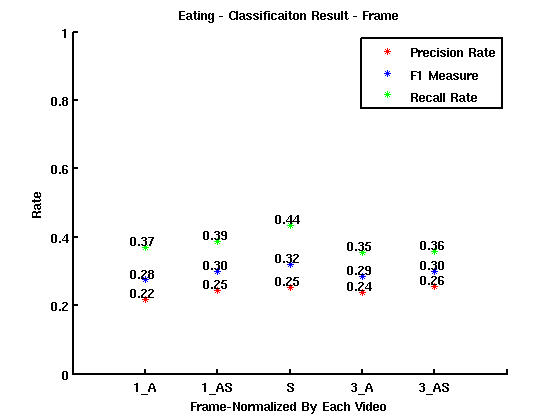
\includegraphics[width=\linewidth]{imgs/Result_Eating_Frame.png}
  \caption{Class Eating - Classification Result of Frame - Frame nomalised by each video}
  \label{fig:REF}
\end{minipage}%
\begin{minipage}{.5\textwidth}
  \centering
  \captionsetup{justification=centering,margin=1cm}
  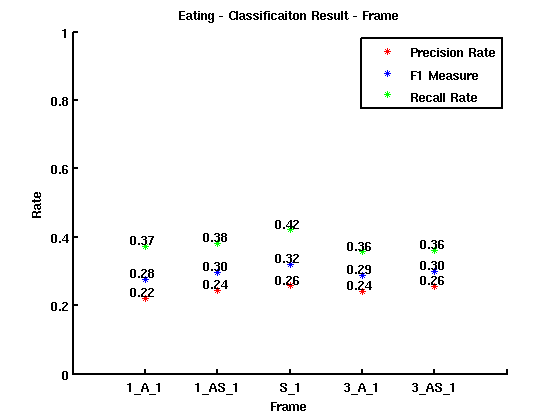
\includegraphics[width=\linewidth]{imgs/Result_Eating_Frame_1.png}
  \caption{Class Eating - Classification Result of Frame - Frame NOT nomalised by each video}
  \label{fig:REF1}
\end{minipage}
\end{figure}

\begin{figure}
\centering
\begin{minipage}{.5\textwidth}
  \centering
  \captionsetup{justification=centering,margin=1cm}
  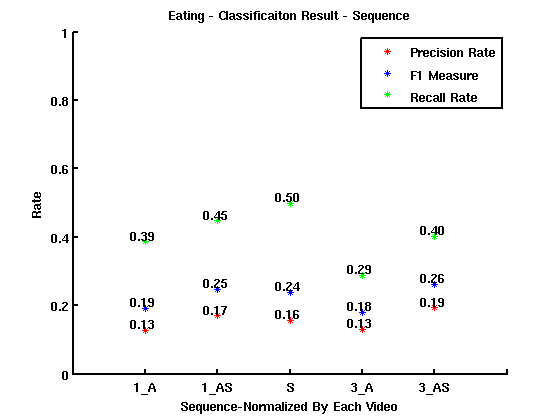
\includegraphics[width=\linewidth]{imgs/Result_Eating_Sequence.png}
  \caption{Class Eating - Classification Result of Frame - Frame nomalised by each video}
  \label{fig:RES}
\end{minipage}%
\begin{minipage}{.5\textwidth}
  \centering
  \captionsetup{justification=centering,margin=1cm}
  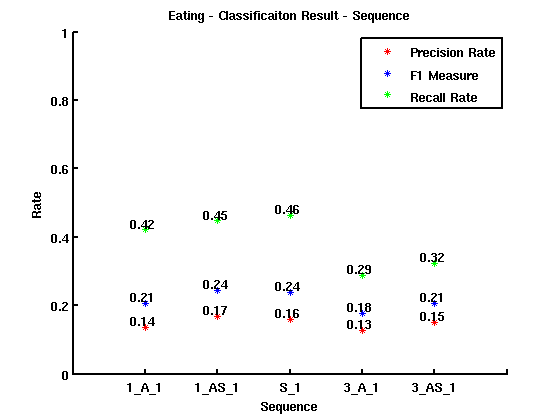
\includegraphics[width=\linewidth]{imgs/Result_Eating_Sequence_1.png}
  \caption{Class Eating - Classification Result of Frame - Frame NOT nomalised by each video}
  \label{fig:RES1}
\end{minipage}
\end{figure}

\begin{figure}
\centering
\begin{minipage}{.5\textwidth}
  \centering
  \captionsetup{justification=centering,margin=1cm}
  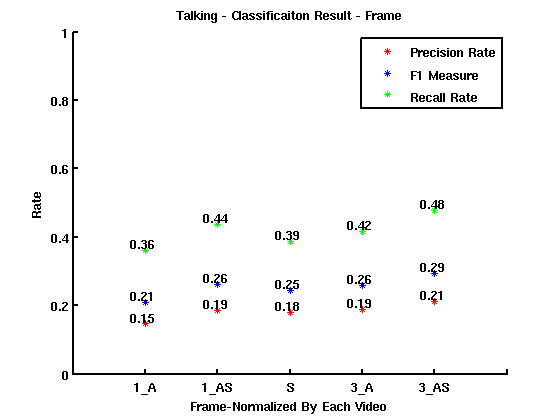
\includegraphics[width=\linewidth]{imgs/Result_Talking_Frame.png}
  \caption{Class Talking - Classification Result of Frame - Frame nomalised by each video}
  \label{fig:RTF}
\end{minipage}%
\begin{minipage}{.5\textwidth}
  \centering
  \captionsetup{justification=centering,margin=1cm}
  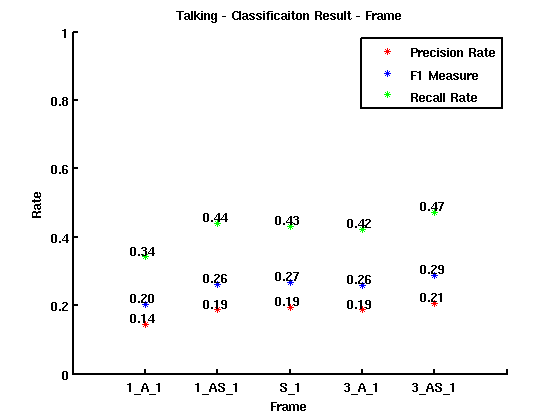
\includegraphics[width=\linewidth]{imgs/Result_Talking_Frame_1.png}
  \caption{Class Talking - Classification Result of Frame - Frame NOT nomalised by each video}
  \label{fig:RTF1}
\end{minipage}
\end{figure}

\begin{figure}
\centering
\begin{minipage}{.5\textwidth}
  \centering
  \captionsetup{justification=centering,margin=1cm}
  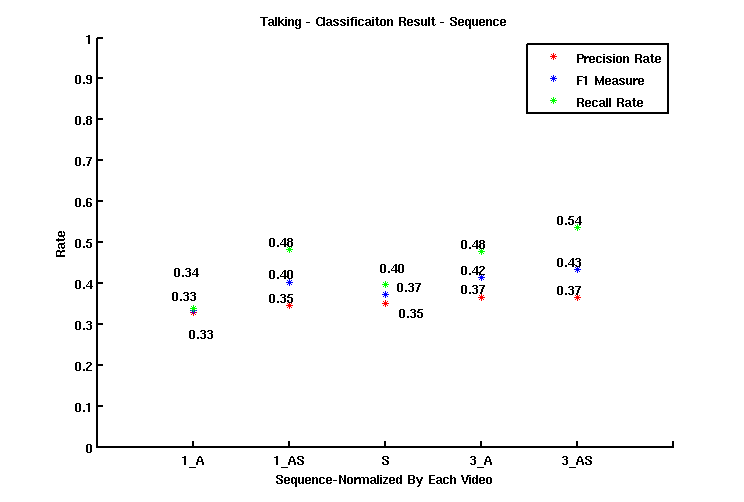
\includegraphics[width=\linewidth]{imgs/Result_Talking_Sequence.png}
  \caption{Class Talking - Classification Result of Sequence - Frame nomalised by each video}
  \label{fig:RTS}
\end{minipage}%
\begin{minipage}{.5\textwidth}
  \centering
  \captionsetup{justification=centering,margin=1cm}
  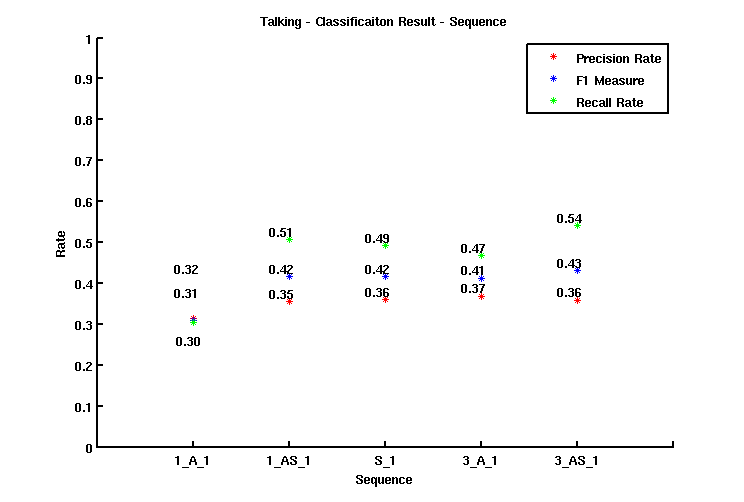
\includegraphics[width=\linewidth]{imgs/Result_Talking_Sequence_1.png}
  \caption{Class Talking - Classification Result of Sequence - Frame NOT nomalised by each video}
  \label{fig:RTS1}
\end{minipage}
\end{figure}

\begin{figure}
\centering
\begin{minipage}{.5\textwidth}
  \centering
  \captionsetup{justification=centering,margin=1cm}
  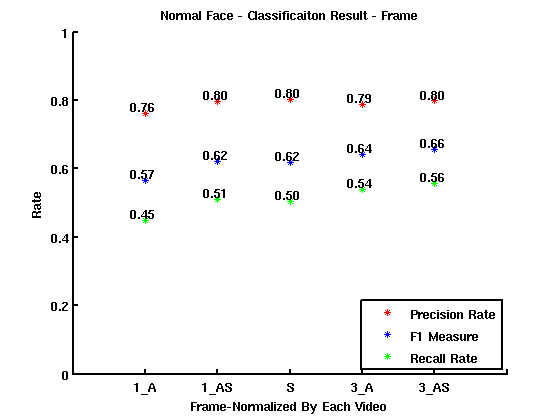
\includegraphics[width=\linewidth]{imgs/Result_NormalFace_Frame.png}
  \caption{Class Normal Face - Classification Result of Frame - Frame nomalised by each video}
  \label{fig:RNF}
\end{minipage}%
\begin{minipage}{.5\textwidth}
  \centering
  \captionsetup{justification=centering,margin=1cm}
  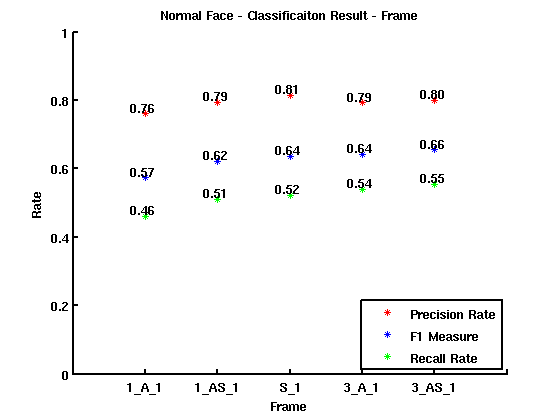
\includegraphics[width=\linewidth]{imgs/Result_NormalFace_Frame_1.png}
  \caption{Class Normal Face - Classification Result of Frame - Frame NOT nomalised by each video}
  \label{fig:RNF1}
\end{minipage}
\end{figure}

\begin{figure}
\centering
\begin{minipage}{.5\textwidth}
  \centering
  \captionsetup{justification=centering,margin=1cm}
  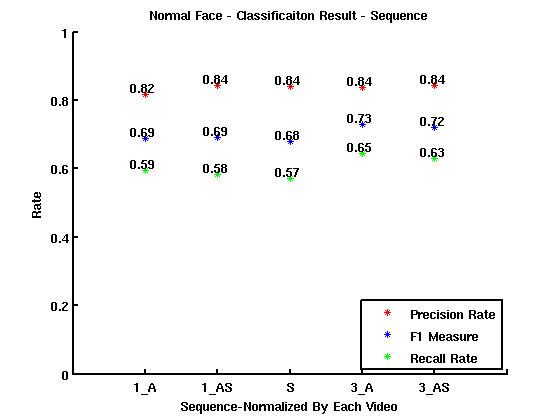
\includegraphics[width=\linewidth]{imgs/Result_NormalFace_Sequence.png}
  \caption{Class Normal Face - Classification Result of Sequence - Frame nomalised by each video}
  \label{fig:RNS}
\end{minipage}%
\begin{minipage}{.5\textwidth}
  \centering
  \captionsetup{justification=centering,margin=1cm}
  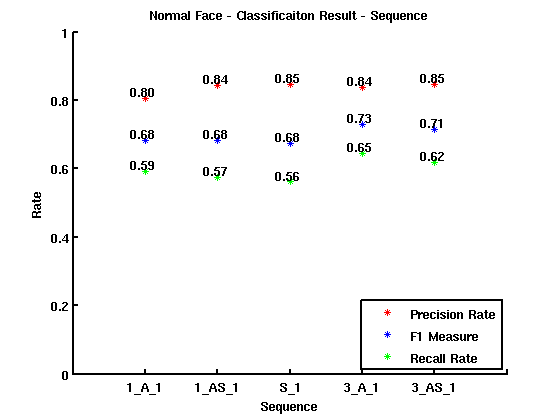
\includegraphics[width=\linewidth]{imgs/Result_NormalFace_Sequence_1.png}
  \caption{Class Normal Face - Classification Result of Sequence - Frame NOT nomalised by each video}
  \label{fig:RNS1}
\end{minipage}
\end{figure}

\begin{figure}
\centering
\begin{minipage}{.5\textwidth}
  \centering
  \captionsetup{justification=centering,margin=1cm}
  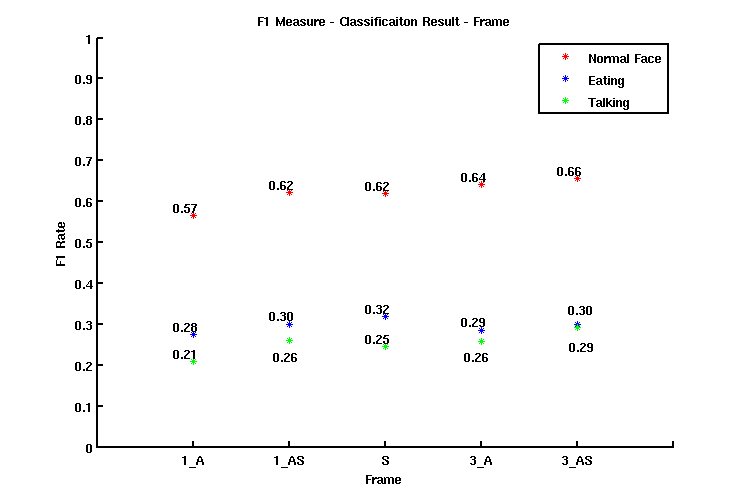
\includegraphics[width=\linewidth]{imgs/Result_F1_Frame.png}
  \caption{Three Class - Classification Result of frame - Frame nomalised by each video}
  \label{fig:RFF}
\end{minipage}%
\begin{minipage}{.5\textwidth}
  \centering
  \captionsetup{justification=centering,margin=1cm}
  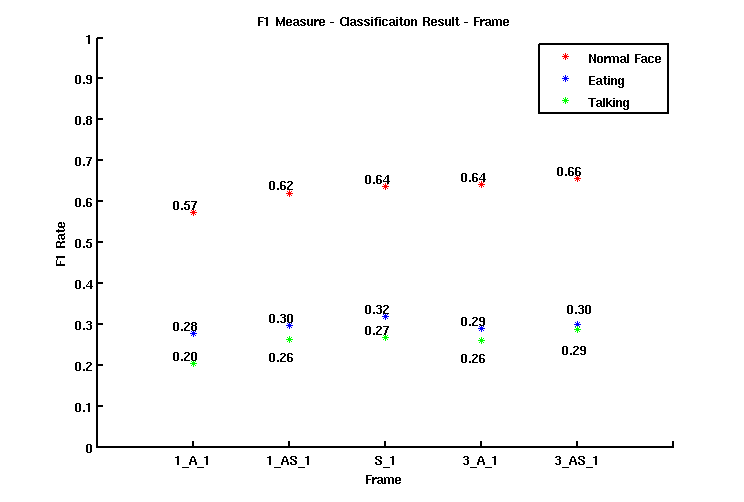
\includegraphics[width=\linewidth]{imgs/Result_F1_Frame_1.png}
  \caption{Three Class - Classification Result of frame - Frame NOT nomalised by each video}
  \label{fig:RFF1}
\end{minipage}
\end{figure}

\begin{figure}
\centering
\begin{minipage}{.5\textwidth}
  \centering
  \captionsetup{justification=centering,margin=1cm}
  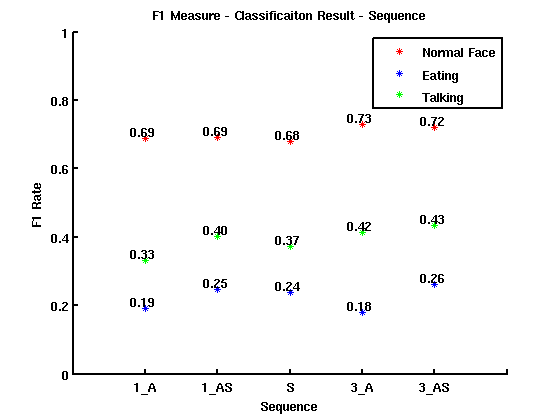
\includegraphics[width=\linewidth]{imgs/Result_F1_Sequence.png}
  \caption{Three Class - Classification Result of frame - Frame nomalised by each video}
  \label{fig:RFS}
\end{minipage}%
\begin{minipage}{.5\textwidth}
  \centering
  \captionsetup{justification=centering,margin=1cm}
  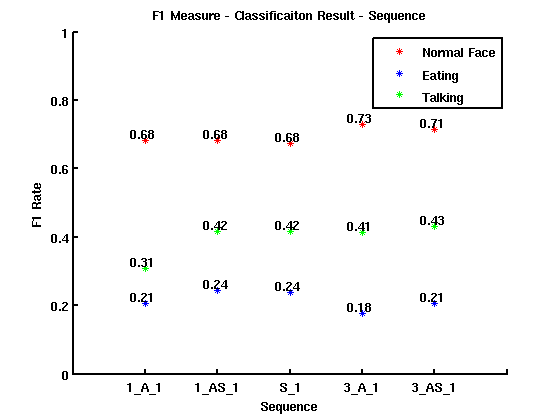
\includegraphics[width=\linewidth]{imgs/Result_F1_Sequence_1.png}
  \caption{Three Class - Classification Result of frame - Frame NOT nomalised by each video}
  \label{fig:RFS1}
\end{minipage}
\end{figure}